\documentclass[uplatex,dvipdfmx,a4paper,10pt]{jsarticle}
\usepackage{graphicx}
\usepackage{amsmath}
\usepackage{latexsym}
\usepackage{multirow}
\usepackage{url}
\usepackage[separate-uncertainty]{siunitx}
\usepackage{physics}
\usepackage{enumerate}
\usepackage{bm}
\usepackage{pdfpages}
\usepackage{pxchfon}
\usepackage{tikz}
\usepackage{float}
\usepackage{listings}
\usepackage{amsmath}
\usepackage{amssymb}
\usepackage{amsfonts}

% lstlistingのsetting
\lstset{
    basicstyle={\ttfamily},
    identifierstyle={\small},
    commentstyle={\smallitshape},
    keywordstyle={\small\bfseries},
    ndkeywordstyle={\small},
    stringstyle={\small\ttfamily},
    frame={tb},
    breaklines=true,
    columns=[l]{fullflexible},
    numbers=left,
    xrightmargin=0zw,
    xleftmargin=3zw,
    numberstyle={\scriptsize},
    stepnumber=1,
    numbersep=1zw,
    lineskip=-0.5ex
}

% tikz setting
\usepackage{tikz}
\usetikzlibrary{automata, intersections, calc, arrows, positioning, arrows.meta}

% theories setting (for japanese language)
\usepackage{amsmath}
\usepackage{amsthm}

\theoremstyle{definition}
\newtheorem{thm}{定理}[section]
\newtheorem{lem}[thm]{補題}
\newtheorem{prop}[thm]{命題}
\newtheorem{cor}[thm]{系}
\newtheorem{ass}[thm]{仮定}
\newtheorem{conj}[thm]{予想}
\newtheorem{dfn}[thm]{定義}
\newtheorem{rem}[thm]{注}

\newtheorem*{thm*}{定理}
\newtheorem*{lem*}{補題}
\newtheorem*{prop*}{命題}
\newtheorem*{cor*}{系}
\newtheorem*{ass*}{仮定}
\newtheorem*{conj*}{予想}
\newtheorem*{dfn*}{定義}
\newtheorem*{rem*}{注}

% \renewcommand{\rmdefault}{pplj}
% \renewcommand{\sfdefault}{phv}

\setlength{\textwidth}{165mm} %165mm-marginparwidth
\setlength{\marginparwidth}{40mm}
\setlength{\textheight}{225mm}
\setlength{\topmargin}{-5mm}
\setlength{\oddsidemargin}{-3.5mm}
% \setlength{\parindent}{0pt}

\def\vector#1{\mbox{\boldmath $#1$}}
\newcommand{\AmSLaTeX}{%
 $\mathcal A$\lower.4ex\hbox{$\!\mathcal M\!$}$\mathcal S$-\LaTeX}
\newcommand{\PS}{{\scshape Post\-Script}}
\def\BibTeX{{\rmfamily B\kern-.05em{\scshape i\kern-.025em b}\kern-.08em
 T\kern-.1667em\lower.7ex\hbox{E}\kern-.125em X}}
\newcommand{\DeLta}{{\mit\Delta}}
\renewcommand{\d}{{\rm d}}
\def\wcaption#1{\caption[]{\parbox[t]{100mm}{#1}}}
\def\rm#1{\mathrm{#1}}
\def\tempC{^\circ \rm{C}}

\makeatletter
\def\section{\@startsection {section}{1}{\z@}{-3.5ex plus -1ex minus -.2ex}{2.3ex plus .2ex}{\Large\bf}}
\def\subsection{\@startsection {subsection}{2}{\z@}{-3.25ex plus -1ex minus -.2ex}{1.5ex plus .2ex}{\normalsize\bf}}
\def\subsubsection{\@startsection {subsubsection}{3}{\z@}{-3.25ex plus -1ex minus -.2ex}{1.5ex plus .2ex}{\small\bf}}
\makeatother

\makeatletter
\def\@seccntformat#1{\@ifundefined{#1@cntformat}%
   {\csname the#1\endcsname\quad}%      default
   {\csname #1@cntformat\endcsname}%    enable individual control
}

% proof enviroment
\renewenvironment{proof}[1][\proofname]{\par
  \pushQED{\qed}%
  \normalfont \topsep6\p@\@plus6\p@\relax
  \trivlist
  \item\relax
  {\bfseries
  #1\@addpunct{.}}\hspace\labelsep\ignorespaces
}{%
  \popQED\endtrivlist\@endpefalse
}
\makeatother

\newcommand{\tenexp}[2]{#1\times10^{#2}}


\begin{document}
% タイトル
\begin{center}
{\Large{\bf 数理計画法 第1回演習課題}} \\
{\bf 電気通信大学 Ⅰ類 コンピュータサイエンスプログラム 3年} \\
{\bf 2311081 木村慎之介} \\
\end{center}

\section{必須課題}
\subsection{問題1}
\begin{itemize}
    \item 許容解: 最適化問題において、集合\(S\)の要素\(\bm{x}\)のこと。
    \item 目的関数: 最適化問題において、最大化したい関数\(f(\bm{x})\)のこと。
    \item 最適解: 任意の\(\bm{x} \in S\)に対して\(f(\bm{x}) \geq f(\bm{x}^*)\)となる許容解\(\bm{x}^*\)のこと。
    \item 最適値: 目的関数値の上界の最小値。
\end{itemize}

\subsection{問題2}
\subsubsection{(a)}
\hspace{1em}\((x, y) = (6, -6)\)を条件式の左辺に代入して計算すると

\begin{equation}
    3 \times 6 +2 \times (-2) = 6
\end{equation}

\noindent となり、条件式の右辺の値に一致するため\((6, -6)\)はこの最適化問題の許容解である。

\subsubsection{(b)}
\hspace{1em}\((x, y) = (0, 3)\)とすると、\(0^2 + 3^2 = 9\)で目的関数値をとり、かつ\(3 \times 0 + 2 \times 3 = 6\)で条件も満たすため、これが題意を満たす許容解の1つである。

\subsubsection{(c)}
\hspace{1em}\(x^2 + y^2  = k^2\)とおくと、最適化問題は条件\(3x + 2y = 6\)を満たしたうえで\(k^2\)を最小化するような\(\bm{x}\)を見つける問題になる。 \\
\hspace{1em}さて、\(x^2 + y^2 = k^2\)は\(x-y\)平面上の原点中心で半径が\(k\)の円を表している。
したかって求める\(k\)の値は原点から直線\(3x + 2y = 6\)への距離の値に等しい。
点と距離の直線公式を用いると\(k\)の値は

\begin{align}
    k   &= \frac{|3 \times 0 + 2 \times 0 - 6|}{\sqrt{3^2 + 2^2}} \\
        &= \frac{6}{\sqrt{13}}
\end{align}

\noindent であるから最適値は\(k^2 = \frac{36}{13}\)と求まる。 \\
\hspace{1em}次に最適値を与える最適解を求める。
最適解を求めるには以下の連立方程式を解けば良い。

\begin{equation} 
    \left\{ \,
        \begin{aligned}
            &   x^2 + y^2 = \frac{36}{13} \\
            &   3x + 2y = 6
        \end{aligned}
    \right.
\end{equation}

\noindent 2つ目の式を\(y\)について整理して1つ目の式に代入すると\(x\)は次のように求まる。

\begin{align}
    x^2 + \left(-\frac{3}{2}x + 3\right)^2  &= \frac{36}{13}    \\
    \left(x - \frac{18}{13}\right)^2        &= 0                \\
    x                                       &= \frac{18}{13}
\end{align}

\noindent 次に連立方程式の2式目に得られた\(x\)の値を代入して\(y\)の値を求めると\(y = \frac{12}{13}\)となる。
よって、最適解は\(\left(x, y\right) = \left(\frac{18}{13}, \frac{12}{13}\right)\)となる。

\subsection{問3}
\hspace{1em}(b)がありえない。

\subsection{問4}
\subsubsection{定式化}
\hspace{1em}製品Ⅰを\(x\)単位、製品Ⅱを\(y\)単位生産すると設定すると、最適化問題は以下のように定式化できる。

\begin{equation}
    \left\{ \,
        \begin{aligned}
            & \text{目的関数: } 3x + 2y \\
            & \text{条件1: } 5x + y \leq 10 \\
            & \text{条件2: } x + 2y \leq 5 \\
            & \text{条件3: } x, y \geq 0
        \end{aligned}
    \right.\
\end{equation}

\subsubsection{実行可能領域の図示}
\hspace{1em}以上の定式化をもとにこの最適化問題の実行可能領域を図示すると以下のようになる。

\begin{figure}[H]
    \centering
    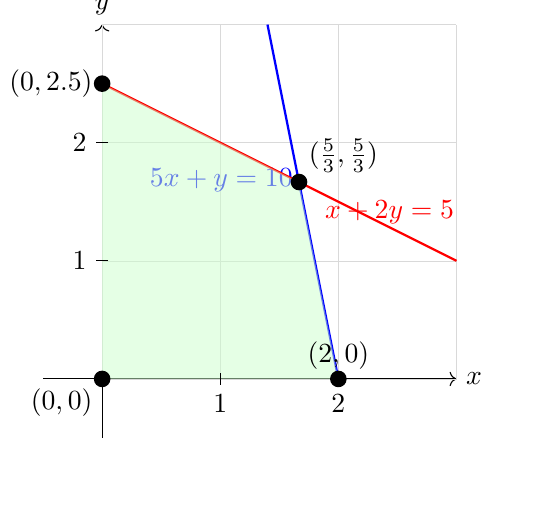
\begin{tikzpicture}[scale=1.5]
        % 軸の描画
        \draw[->] (-0.5,0) -- (3,0) node[right] {$x$};
        \draw[->] (0,-0.5) -- (0,3) node[above] {$y$};
        
        % グリッド
        \draw[help lines, gray!30] (0,0) grid (3,3);
        
        % 制約条件の直線
        % 条件1: 5x + y = 10 → y = 10 - 5x
        \draw[thick, blue] (1.4,3) -- (2,0) node[pos=0.5, above left] {$5x + y = 10$};
        
        % 条件2: x + 2y = 5 → y = (5-x)/2
        \draw[thick, red] (0,2.5) -- (3,1) node[pos=0.6, below right] {$x + 2y = 5$};
        
        % 実行可能領域の塗りつぶし
        \fill[green!20, opacity=0.5] (0,0) -- (0,2.5) -- (1.667,1.667) -- (2,0) -- cycle;
        
        % 頂点の描画
        \fill (0,0) circle (2pt) node[below left] {$(0,0)$};
        \fill (0,2.5) circle (2pt) node[left] {$(0,2.5)$};
        \fill (2,0) circle (2pt) node[above] {$(2,0)$};
        \fill (1.667,1.667) circle (2pt) node[above right] {$(\frac{5}{3},\frac{5}{3})$};
        
        % 座標軸の目盛り
        \foreach \x in {1,2}
            \draw (\x,0.05) -- (\x,-0.05) node[below] {\x};
        \foreach \y in {1,2}
            \draw (0.05,\y) -- (-0.05,\y) node[left] {\y};
    \end{tikzpicture}
    \caption{実行可能領域}
\end{figure}

\section{問2}
\subsection{(1)}
\hspace{1em}作成したプログラムを以下に乗せる。

\begin{lstlisting}[caption={最小二乗推定量と正則化最小二乗推定量を求めるプログラム}, label={code_regression}]
# Print the first 6 rows of the data used for analysis
print("--- 分析に使用するデータ(dat)の先頭6行 ---")
print(head(dat))

# OLS and Ridge regression
beta_ols <- solve(t(X) %*% X) %*% t(X) %*% y

rownames(beta_ols) <- c("Intercept", "x1", "x2", "x3", "x4", "x5", "x6")
colnames(beta_ols) <- "OLS_estimate"

lambda <- 1
p <- ncol(X)
I <- diag(p)

I[1, 1] <- 0

# Ridge regression
beta_ridge <- solve(t(X) %*% X + lambda * I) %*% t(X) %*% y

rownames(beta_ridge) <- c("Intercept", "x1", "x2", "x3", "x4", "x5", "x6")
colnames(beta_ridge) <- "Ridge_estimate"

# Output results
print("--- 最小二乗推定量 (OLS) ---")
print(beta_ols)

print("--- 正則化最小二乗推定量 (Ridge, λ=1) ---")
print(beta_ridge)
\end{lstlisting}

次に、実行結果を以下に乗せる。

\begin{lstlisting}[caption={コード\ref{code_regression}の実行結果}, label={code_output_regression}]
[1] "--- 分析に使用するデータ(dat)の先頭6行 ---"
                    x1         x2         x3         x4         x5        x6
Courtelary   0.8051305 -1.4820682  0.1062125 -0.7477267 0.77503669 0.8029583
Delemont     1.0372847 -0.2447942 -0.2057867  1.0477479 0.77503669 1.0359411
Franches-Mnt 1.7897846 -0.4825622 -0.6217858  1.2529998 0.08838778 1.7899671
Moutier      1.2534283 -0.6234617 -0.4137863 -0.1768099 0.12272023 1.2563525
Neuveville   0.5409551 -0.3152440  0.4182118 -0.8628212 0.22571757 0.5383002
Porrentruy   0.4769125 -0.6762990 -0.4137863  1.1851420 2.28566429 0.4798413
                       y
Courtelary   -0.18668632
Delemont     -1.31480509
Franches-Mnt -1.44015162
Moutier      -0.56272591
Neuveville    0.06400674
Porrentruy   -0.93876550
[1] "--- 最小二乗推定量 (OLS) ---"
           OLS_estimate
Intercept  3.760880e-15
x1        -2.708939e+01
x2        -2.317531e-01
x3         3.924185e-01
x4        -3.545175e-01
x5         3.419800e-02
x6         2.693602e+01
[1] "--- 正則化最小二乗推定量 (Ridge, λ=1) ---"
          Ridge_estimate
Intercept   1.266348e-16
x1         -8.695476e-02
x2         -2.450151e-01
x3          3.738593e-01
x4         -3.382417e-01
x5          3.664733e-02
x6         -8.079264e-02
\end{lstlisting}

結果を確認すると、\(x_1\)と\(x_6\)の係数において、最小二乗推定量では絶対値が大きくなっているのに対して、正則化最小二乗推定量は絶対値が他の回帰係数と差が無いことが読み取れる。
これは多重共線性が影響していると考えられる。

結果\ref{code_output_regression}の入力データの部分を見ると、\(x_1\)と\(x_6\)に相関関係が見られる。
相関が大きいデータがあると逆行列を求める際に、相関が高い部分の係数の値が大きくなってしまう。

一方、正則化最小二乗推定量ではこの相関が高くなってしまった時でも逆行列を求める際に、相関が高いところでもある程度値を抑える役割があるため、極端に大きな値にはならなかった。

\subsection{(2)}
以下に各回帰係数の検定を行うために実装したコードを乗せる。

\begin{lstlisting}[caption={回帰係数の検定プログラム}, label={code_check}]
# Remove the 6th column (x6) from the data
dat_rm <- dat[, -6]

# Prepare the explanatory variables as a matrix (x1 to x5)
x <- as.matrix(dat_rm[, 1:5])

# Run the linear model (lm) and output the summary of the results
model_summary <- summary(lm(y ~ x))

# Print the summary of the linear model
print(model_summary)
\end{lstlisting}

この出力結果は以下のようになった。

\begin{lstlisting}[caption={コード\ref{code_check}の実行結果}, label={code_output_check}]
Call:
lm(formula = y ~ x)

Residuals:
     Min       1Q   Median       3Q      Max 
-1.13350 -0.35713 -0.06654  0.38179  0.86331 

Coefficients:
              Estimate Std. Error t value Pr(>|t|)   
(Intercept)  1.352e-16  7.959e-02   0.000  1.00000   
xx1         -1.491e-01  1.467e-01  -1.016  0.31546   
xx2         -2.350e-01  1.249e-01  -1.881  0.06705 . 
xx3          3.982e-01  1.550e-01   2.569  0.01392 * 
xx4         -3.543e-01  1.102e-01  -3.215  0.00254 **
xx5          3.552e-02  9.236e-02   0.385  0.70250   
---
Signif. codes:  0 ‘***’ 0.001 ‘**’ 0.01 ‘*’ 0.05 ‘.’ 0.1 ‘ ’ 1

Residual standard error: 0.5457 on 41 degrees of freedom
Multiple R-squared:  0.7346,    Adjusted R-squared:  0.7022 
F-statistic:  22.7 on 5 and 41 DF,  p-value: 7.624e-11
\end{lstlisting}

まず実行結果のcoefficientsを確認するとPrがp値を求めていることが分かる。
ここを確認すると0.05より小さいのは\(x_3\)と\(x_4\)であることが分かる。

また、回帰全体の有効性を確認するには最後の行を確認すれば良い。
これによると、p値が0.05を大きく下回っているため少なくとも1つの回帰係数は有意差を持っていることが分かる。

\subsection{(3)}
以下に実装したプログラムを乗せる。


%%%%%%%%%%%%%%%%%%%%%%%%%%%%%%%%%%%%%%%%%%%%%%%%%%%%%%%%%%%%%%%%%%%%%%
\appendix
\setcounter{figure}{0}
\setcounter{table}{0}
\numberwithin{equation}{section}
\renewcommand{\thetable}{\Alph{section}\arabic{table}}
\renewcommand{\thefigure}{\Alph{section}\arabic{figure}}
%\def\thesection{付録\Alph{section}}
\makeatletter 
\newcommand{\section@cntformat}{付録 \thesection:\ }
\makeatother
%%%%%%%%%%%%%%%%%%%%%%%%%%%%%%%%%%%%%%%%%%%%%%%%%%%%%%%%%%%%%%%%%%%%%%

    
\end{document}